\documentclass[12pt]{amsart}
\usepackage[margin = 1in]{geometry}
\usepackage{amsmath, amssymb, amsthm, graphicx}
\usepackage{enumerate}
\usepackage[all]{xy}
\usepackage{mathrsfs}

%%%%%%%%%%%%%% COLOR COMMENTS! %%%%%%%%%%%%%%%
\usepackage{color}
\newcommand{\dzb}[1]{{\color{blue} \sf
    $\spadesuit\spadesuit\spadesuit$ DZB: [#1]}}
\newcommand{\reword}[1]{{\color{red} \sf $\spadesuit\spadesuit\spadesuit$ reword: [#1]}}

% changed above definition to make comments disappear
%\newcommand{dzb}[1]{}
%\newcommand{reword}[1]{}

% Color names: http://en.wikibooks.org/wiki/LaTeX/Colors#The_68_standard_colors_known_to_dvips
\usepackage[usenames,dvipsnames]{xcolor}
\newcommand{\note}[1]{{\color{BurntOrange} $\blacktriangle\blacktriangle$\sf Note: [#1]}}

\newcommand{\F}[0]{\mathbb{F}}
\newcommand{\tr}[0]{\operatorname{tr}}
\newcommand{\wt}[1]{\widetilde{#1}}
\newcommand{\frob}[0]{\operatorname{Frob}}
\newcommand{\card}[0]{\#}
\newcommand{\pmat}[4]{\begin{pmatrix}#1 & #2 \\ #3 & #4\end{pmatrix}}
\newcommand{\pderiv}[2]{\frac{\partial #1}{\partial #2}}
\newcommand{\Ov}{\mathcal{O}_{v}}
\newcommand{\Ok}{\mathcal{O}_{K}}
\newcommand{\Q}{\mathbb{Q}}
\newcommand{\Z}{\mathbb{Z}}
\newcommand{\C}{\mathbb{C}}
\newcommand{\leg}[2]{\left(\frac{#1}{#2}\right)}
\newcommand{\calO}{\mathcal{O}}
\newcommand{\frakp}{\mathfrak{p}}
\newcommand{\frakq}{\mathfrak{q}}
\newcommand{\mf}[1]{\mathfrak{#1}}
\newcommand{\nm}{\operatorname{N}_{K/\Q}}
\newcommand{\Cl}{\operatorname{Cl}}
\newcommand{\oo}{\mathcal{O}}
\newcommand{\sgn}{\operatorname{sgn}}
\newcommand{\Gal}{\operatorname{Gal}}
\newcommand{\cl}{\overline}
\newcommand{\mc}[1]{\mathcal{#1}}
\newcommand{\Cc}{\mathcal{C}}
\newcommand{\Dc}{\mathcal{D}}
\newcommand{\raym}{\mathcal{C}^{\frakm}_K}
\newcommand{\frakr}{\mathfrak{r}}
\newcommand{\Spec}{\text{Spec} \ }
\newcommand{\Hom}{\text{Hom}}
\newcommand{\ord}{\text{ord}}
\newcommand{\scr}[1]{\mathscr{#1}}
\newcommand{\R}{\mathbb{R}}
\newcommand{\cal}[1]{\mathcal{#1}}
\newcommand{\Nm}{\text{Nm}}
\newcommand{\A}{\mathbb{A}}
\newcommand{\ti}{\times}
\newcommand{\Hbb}{\mathbb{H}}
\newcommand{\mbf}[1]{\mathbf{#1}}
%\newcommand{\leg}[2]{\left(\frac{ \# 1}{\# 2} \right)}

\DeclareMathOperator{\GL}{GL}
\DeclareMathOperator{\SL}{SL}
\DeclareMathOperator{\Frob}{Frob}
\DeclareMathOperator{\ab}{ab}
\DeclareMathOperator{\cyc}{cyc}
\DeclareMathOperator{\N}{N}
\DeclareMathOperator{\Ver}{Ver}
\DeclareMathOperator{\Art}{Art}
\DeclareMathOperator{\Spl}{Spl}
\DeclareMathOperator{\sep}{sep}
\DeclareMathOperator{\Stab}{Stab}
\DeclareMathOperator{\Sp}{Sp}
\DeclareMathOperator{\SO}{SO}
\DeclareMathOperator{\SU}{SU}
\DeclareMathOperator{\PGL}{PGL}
\DeclareMathOperator{\Mat}{Mat}
\DeclareMathOperator{\Tr}{Tr}
\DeclareMathOperator{\End}{End}
\DeclareMathOperator{\Ad}{Ad}
\DeclareMathOperator{\Aut}{Aut}
\DeclareMathOperator{\WPr}{WPr}

\newtheorem{thm}{Theorem}
\newtheorem{lemma}[thm]{Lemma}
\newtheorem{defn}[thm]{Definition}
\newtheorem{prop}[thm]{Proposition}
\newtheorem{cor}[thm]{Corollary}
\newtheorem{ex}[thm]{Example}
\newtheorem{crit}[thm]{Criterion}


\theoremstyle{remark}
\newtheorem{rem}[thm]{Remark}

\makeatletter
\def\imod#1{\allowbreak\mkern5mu({\operator@font mod}\,\,#1)}
\makeatother

\widowpenalty=1000
\clubpenalty=1000

\title{CS 181 Problem Set 2}
\author{Ashok Cutkosky and Tony Feng}


\begin{document}
\maketitle

\noindent \textbf{Problem 1.} It will be useful to note the following property of perceptrons, which will aid us in proving that certain problems are not linearly separable. By including a ``dummy feature'' $x_0$ which always has value $1$, we may assume that hypothesis function is given by 
\[
h_{\mbf{w}}(\mbf{x}) = g(\mbf{x}^T \mbf{w})
\]
Then if $\mbf{x}$ and $\mbf{y}$ are both classified positively, we have $h_{\mbf{w}}(\mbf{x}) >0 $ and $h_{\mbf{w}}(\mbf{y}) > 0$ so $h_{\mbf{w}}(\mbf{x}+\mbf{y}) > 0$ by linearity. 

If problems $\mbf{x}'$ and $\mbf{y}'$ that are both classified negatively, similar logic implies that $h_{\mbf{w}}(\mbf{x}'+\mbf{y}') \leq 0$. We have proved the following: 

\begin{lemma}\label{no_perceptron}
If there exist feature vectors $\mbf{x}, \mbf{y}$ that are classified positively and $\mbf{x}', \mbf{y}'$ that are classified negatively such that $\mbf{x} + \mbf{y} = \mbf{x}' + \mbf{y}'$, then the problem does not admit a solution by a perceptron. 
\end{lemma}

\begin{enumerate}
\item No perceptron can solve this. Indeed, take 
\[
\mbf{x} \leftrightarrow \begin{pmatrix} 1 & 1 & 1 \\ 1 & 1 & 1 \\ 1 & 1 & 1 \end{pmatrix} \hspace{1cm} \mbf{y} \leftrightarrow \begin{pmatrix} -1 & -1 & -1 \\ -1 & -1 & -1 \\ -1 & -1 & -1 \end{pmatrix} 
\]
 and  
\[
\mbf{x} \leftrightarrow \begin{pmatrix} 1 & 1 & 1 \\ 1 & 1 & 1 \\ -1 & -1 & -1 \end{pmatrix} \hspace{1cm} \mbf{y} \leftrightarrow \begin{pmatrix} -1 & -1 & -1 \\ -1 & -1 & -1 \\ 1 & 1 & 1 \end{pmatrix} ,
\]
which fulfill the hypotheses of Lemma \ref{no_perceptron}.

\item We claim that the perceptron with weights indicated by the matrix
\[
\begin{pmatrix} w_{11} = 1 & w_{12} = 1 & w_{13} = 1 \\ w_{21} = \frac{1}{2} & w_{22} = \frac{1}{2} &  w_{23} = \frac{1}{2}  \\ w_{31} = \frac{1}{2} & w_{32} = \frac{1}{2} & w_{33} = \frac{1}{2}  \end{pmatrix}
\]
classifies this problem. Indeed, suppose that there are $a$ ``on'' pixels in the top row and $b$ ``on'' pixes in the bottom two rows. Then $\mbf{w}^T  x = a - (3-a) + \frac{1}{2} (b - (3-b)) = 2a-3  - (b-3) = 2a - b$, which is positive if and only if $2a > b$. On the other hand, the fraction of ``on'' pixels in the top row is $\frac{a}{3}$ and the fraction of ``on'' pixels in the bottom two rows is $\frac{b}{6}$, so the former is larger than the latter if and only if $2a > b$, as desired. 

\item No perceptron can solve this. Indeed, take 
\[
\mbf{x} \leftrightarrow \begin{pmatrix} 1 & -1 & 1 \\ -1 & 1 & -1 \\ 1 & -1 & 1 \end{pmatrix} \hspace{1cm} \mbf{y} \leftrightarrow \begin{pmatrix} -1 & 1 & -1 \\ 1 & -1 & 1 \\ -1 & 1 & -1 \end{pmatrix} 
\]
 and  
\[
\mbf{x} \leftrightarrow \begin{pmatrix} 1 & 1 & 1 \\ 1 & 1 & 1 \\ -1 & -1 & -1 \end{pmatrix} \hspace{1cm} \mbf{y} \leftrightarrow \begin{pmatrix} -1 & -1 & -1 \\ -1 & -1 & -1 \\ 1 & 1 & 1 \end{pmatrix} ,
\]
which fulfill the hypotheses of Lemma \ref{no_perceptron}.
\end{enumerate}



\noindent \textbf{Problem 2.} 
\begin{enumerate}
\item \emph{Decision Trees} are effective when there are a few inputs of great significance. They can represent interesting interactions between inputs, which is useful in identifying idiosyncratic features of certain digits, such as contiguous segments.

However, decision trees are not effective at judging the input holistically, being required to focus on one feature at a time. This seems like a severe problem in digit recognition, where it is the general shape of the figure, rather than the particular input pixels that it occupies, which is important for identification. 

\item \emph{Boosted decision stumps} have the advantage of tending not to overfit, which seems like a real pitfall in the digit classification problem. Digit classification is qualitatively similar to polynomial fitting of data points, so it is conceivable that a learner would be susceptible to overfitting the specific features of the training data. 

However, boosting is essentially a hodgepodge of weak methods, and its effectiveness does depend on the efficacy of these weak learners. We have seen that naive learners struggle to identify features such as connectivity, which is certainly important in digit recognition. 

\item \emph{Perceptrons.} Perceptrons are useful for identifying linear decision boundaries, and can depend on all of the input data. In this way, they are better for holistically judging the input than are decision trees. 

However, they suffer from not being able to identify interesting interactions between the inputs, and such interactions are important in handwriting recognition for the purpose of identifying contiguous segments and loops. 

\item \emph{Multi-layer feed forward Neural Networks} possess much more flexibility and range than perceptrons. They can represent virtually any function of the input, given sufficiently many layers. 

However, the range of expression also makes neural networks vulnerable to overfitting. Regularization, pruning, and other methods should be used to ensure that this does not happen. 
\end{enumerate}

\noindent \textbf{Problem 3.}

\begin{itemize}
\item[1.-4.] See source code.

\item[5.]

\item[6.]
\begin{itemize}
\item[a.] Learning rate 0.05
\item[b.] 

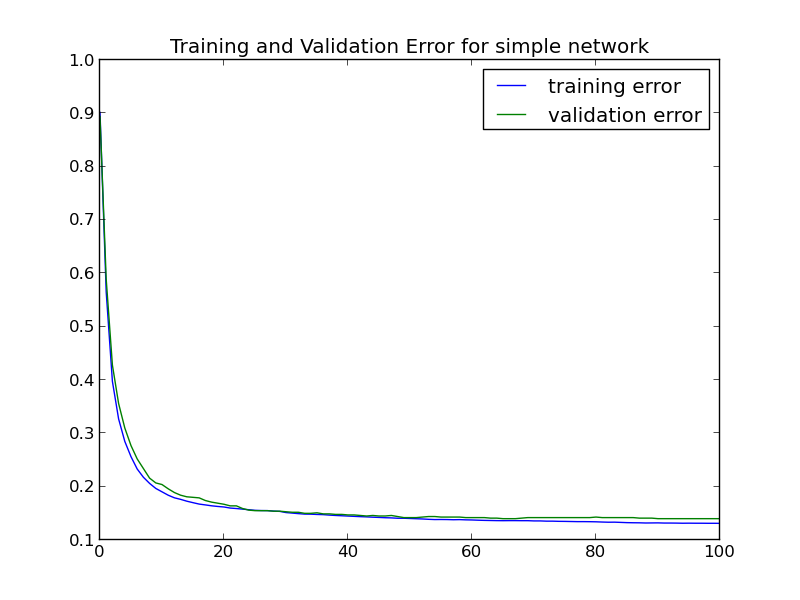
\includegraphics[height =2in]{simple100_005}

60 is a good number of epochs to train for, since validation set error stops decreasing at that point. It is important to use the validation set to tune the number of epochs because the validation set will measure how well our learning on the test set generalizes to other examples, so that we avoid overfitting.

\item[c.] At 60 epochs the training set performance was 0.863 and the validation set performance was 0.858.
\end{itemize}

\item[8.] Our custom network features two hidden layers. The first hidden layer consists of nodes connected 
to connected $3 \times 3$ squares of the image, jumping by intervals of $3$ (so that the squares are 
disconnected). This idea exploits the locality of images - that is, the fact that we should focus on important 
\emph{groups} of pixels rather than individual pixels. It is one of the two important tools from the Le Cun et 
al. paper. The point is that we believe generalizable models should operate at a lower level of resolution.

The second hidden layer is the same as in the simple neural network. We observed that performance peaked 
at about $0.75$, so it was actually worse than the simple neural network. Perhaps our hypothesis about 
locality was wrong. 

\end{itemize}


\noindent \textbf{Problem 4.}

\begin{itemize}

\item[1.]
$C$ is attempting to address the complexity of the network - it is implementing regularization. A network in which many weights are actually zero represents a graph in which some nodes in one layer are actually not connected to nodes in the next layer, which is a simpler scenario than the fully-connected network. The additional summation in $C$ penalizes higher weights so that the network will limit its complexity.

\item[2.]
If our learning rate is $\alpha$, then according to gradient descent, we want the update rule to be 
\[
w_{mj}^{(r+1)} \leftarrow w_{mj}^{(r)} + \alpha \frac{\partial C}{\partial w_{mj}^{(r)}}
\]
Now we have
\[
C=\mathcal{L}+\lambda \sum {w_{mj}}^2
\]
Where the second sum runs over all the weights in the network.
Thus
\[
\frac{\partial C}{\ w_{mj}} = \frac{\partial \mathcal{L}}{\partial w_{mj}}+2\lambda w_{mj}
\]
and 
\[
\frac{\partial C}{\ w_{km}} = \frac{\partial \mathcal{L}}{\partial w_{km}}+2\lambda w_{km}
\]
We already know $\frac{\partial \mathcal{L}}{\partial w_i}$ from the original backprogagation rule. Thus our update rule is
\[
w_{mj}^{(r+1)} \leftarrow w_{mj}^{(r)}+\alpha a_{m}\delta_j-2\alpha\lambda w_{mj}
\]
and analogous for $w_{km}$, just replacing the indices. 
\end{itemize}


\end{document}



